%% -*- coding: utf-8 -*-
\documentclass[12pt,a4paper]{scrartcl} 
\usepackage[utf8]{inputenc}
\usepackage[english,russian]{babel}
\usepackage{indentfirst}
\usepackage{misccorr}
\usepackage{graphicx}
\usepackage{amsmath}
\usepackage{hyperref}

\begin{document}

\author{}
\date{}
\maketitle

\section{Введение}
\label{sec:intro}

При внедрении возобновляемых источников энергии требуется выполнить оценку эффективности конкретных источников на выбранной территории. Во время оценки используется большое количество данных, проводится множество преобразований информации, а потому целесообразно разработать программу, автоматизирующую этот процесс.

В ходе учебной практики была разработана Python-библиотека, которая может быть полезна для оценки энергетического потенциала региона.

\section{Описание библиотеки}
\label{sec:desc}

\subsection{Зависимости}
\label{sec:desc:dep}

Используйте пакетный менеджер pip для установки необходимых зависимостей:

\begin{verbatim}
  pip install -r requirements.txt
\end{verbatim}

При необходимости используйте виртуальное окружение.

\subsection{Использование}
\label{sec:desc:usage}

Пример расчёта распределения энергии для коровьего навоза:

\begin{verbatim}
from edc.energy_source.cow_dung_energy_source import CowDungEnergySource

# Выбор источика энергии
energy_source = CowDungEnergySource()

# Расчёт распределения энергии для выбранного источника энергии.
# Для всех источников используется один и тот же метод.
# path - путь до каталога с необходимыми для расчёта данными
map = energy_source.calculateEnergyGenerationDistribution(path="data")

# Вывод результата
map.draw()
\end{verbatim}

Пример вывода для этого источника энергии:

\begin{verbatim}
Российская Федерация:    754.3 ПДж
Южный федеральный округ: 111.4 ПДж
Республика Адыгея:         2.4 ПДж
Республика Калмыкия:      21.0 ПДж
Республика Крым:           4.3 ПДж
Краснодарский край:       21.0 ПДж
Астраханская область:     15.3 ПДж
Волгоградская область:    18.0 ПДж
Ростовская область:       29.2 ПДж
г. Севастополь:           49.0 ТДж
\end{verbatim}

\subsection{Входные данные}
\label{sec:desc:inpd}

\begin{itemize}
  \item \texttt{data/} - путь для входных данных. При желании можно указать любой другой.
  \item \texttt{data/osm/} - тут могут храниться данные, полученные из OpenStreetMap.
  \item \texttt{data/number\_of\_cows.json} - поголовье коров по данным Росстат на 1 октября 2023 года.
  \item \texttt{data/properties.json} - прочие данные для оценки энергии, получаемой из коровьего навоза.
\end{itemize}

\subsection{Поддерживаемые форматы}
\label{sec:desc:fs}

\begin{itemize}
  \item \texttt{txt}
  \item \texttt{json}
  \item \texttt{shp} (OpenStreetMap): каждому полигону в соответствии ставится его площадь, вычисляемая на эллипсоиде.
\end{itemize}

\subsection{Источники энергии}
\label{sec:desc:es}
\begin{itemize}
  \item Коровий навоз: навоз перерабатывается в метан и сгорает. Оценивается количество вырабатываемой энергии за год. Данные представлены в международной системе единиц (СИ).
  \item Солнце и ветер: добавлены как примеры других источников энергии в целях демонстрации расширения возможностей программы.
  \item \texttt{ExampleOfRasterDistributionEnergySource} - демонстрация вывода распределения энергии в растровом формате.
\end{itemize}

\subsection{Вывод данных}
\label{sec:desc:opd}

Данные могут быть выведены в консоль:
\begin{itemize}
  \item в сыром виде,
  \item в формате ключ-значение.
\end{itemize}

Также возможен вывод растровых и векторных данных. Используется \href{https://github.com/matplotlib/matplotlib}{matplotlib} и другие библиотеки.

Пример вывода растровых данных представлен на рис.~\ref{fig:wex}.
\begin{figure}[h]
  \centering
  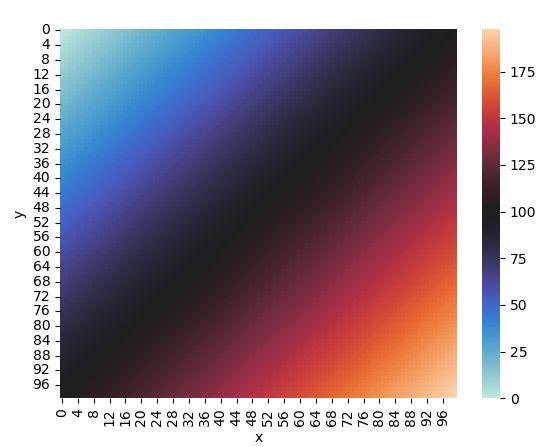
\includegraphics[width=1\textwidth]{raster_distribution.png}
  \caption{Пример вывода растровых данных}\label{fig:wex}
\end{figure}

Пример вывода векторных данных (леса в Южном федеральном округе согласно OpenStreetMap); чем ярче цвет — тем больше площадь полигона, представлен на рис.~\ref{fig:wexx}.
\begin{figure}[h]
  \centering
  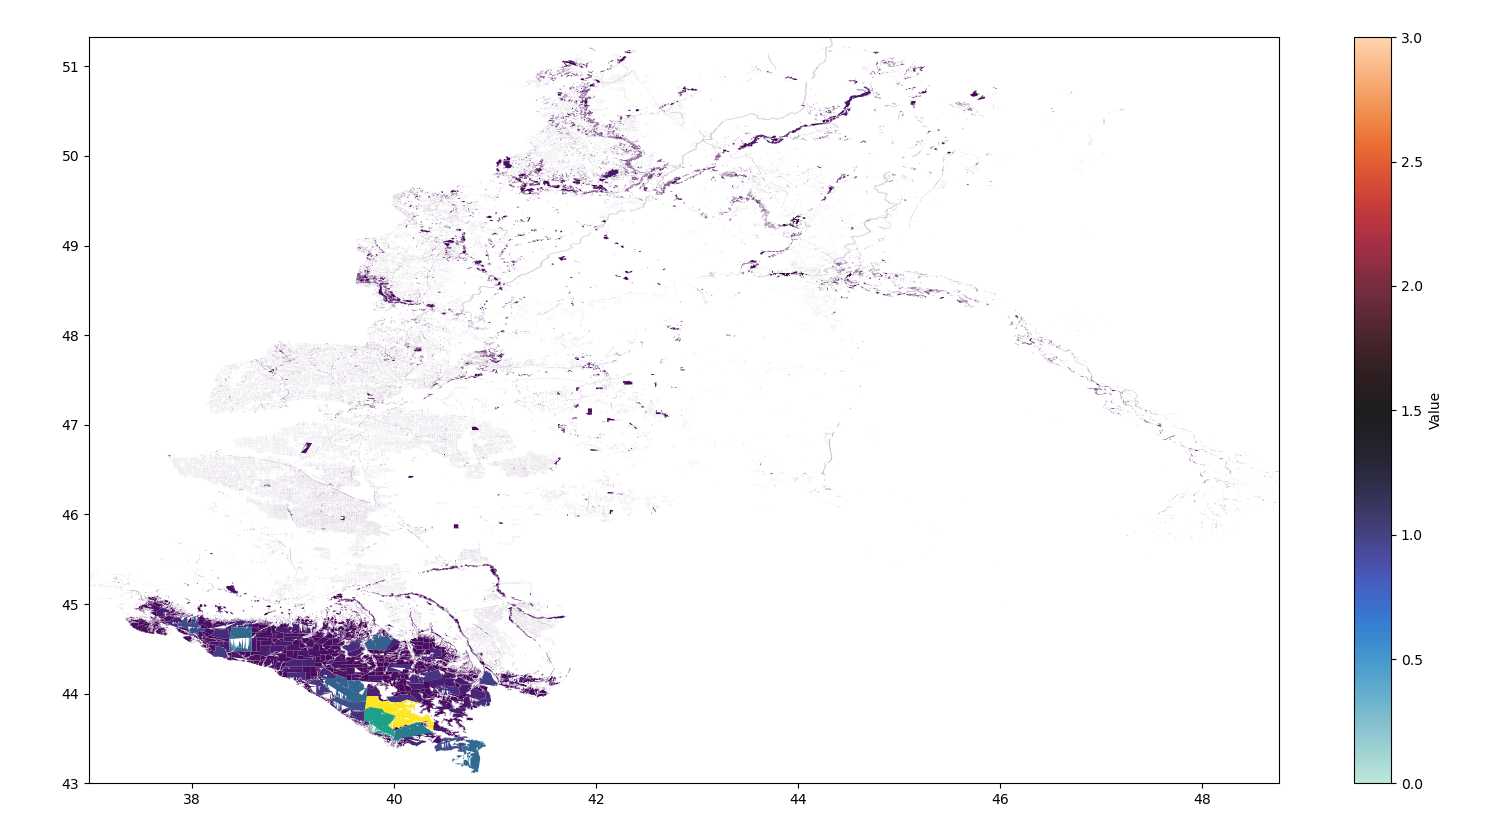
\includegraphics[width=1\textwidth]{vector_distribution.png}
  \caption{Пример вывода векторных данных}\label{fig:wexx}
\end{figure}

\subsection{Методика расчёта для демонстрационного примера с получением энергии из коровьего навоза}
\label{sec:desc:cm}

Поголовье коров по данным Росстат на 1 октября 2023 года:

\begin{verbatim}
  Российская Федерация                7.7 млн
  Южный федеральный округ          1136.8 тыс
  Республика Адыгея                  24.6 тыс
  Республика Калмыкия               214.7 тыс
  Республика Крым                    44.2 тыс
  Краснодарский край                214.4 тыс
  Астраханская область              156.2 тыс
  Волгоградская область             184.2 тыс
  Ростовская область                298.1 тыс
  г. Севастополь                      0.5 тыс
\end{verbatim}

Эти данные представлены в \texttt{data/number\_of\_cows.json}.

Условно (для реальных данных может отличаться):

\begin{verbatim}
  Корова массой 450 кг;
  Производит 8% от массы коровы навоза в сутки = 36 кг;
  Выход биогаза на кг навоза: 0.4 м^3;
  Содержание метана в биогазе 65%;
  Плотность метана 0.714 кг/м^3;
  Удельная теплота сгорания метана 50.2 МДж/кг;
  При сгорании метана остаётся 80% полезной энергии (тепло);
\end{verbatim}

Эти данные представлены в \texttt{data/properties.json}.

Имеем:
\begin{itemize}
  \item 13 т навоза в год на одну корову.
\end{itemize}

На одну корову в сутки:
\begin{itemize}
  \item Количество биогаза в сутки: 14.4 м\(^3\).
  \item Объём метана в сутки: 9.36 м\(^3\).
  \item Масса метана: 6.7 кг.
  \item Энергия, выделяемая при сгорании метана: 335.5 МДж.
  \item С учётом потерь, полезная энергия: 270 МДж.
\end{itemize}

Количество полезной энергии в год:
\begin{itemize}
  \item На одну корову: 98 ГДж.
  \item На всех коров в Республике Адыгея: 2410 ТДж.
\end{itemize}

Если всю эту теплоту преобразовать в электроэнергию с КПД 40\%, получим:
\begin{itemize}
  \item 268 млн кВт\(\cdot\)ч электроэнергии в год.
\end{itemize}

Для сравнения:
\begin{itemize}
  \item Мощность Майкопской ГЭС — 9.4 МВт.
  \item Среднегодовая выработка — 48.4 млн кВт\(\cdot\)ч.
\end{itemize}

Стоит отметить, что производственный цикл также требует энергии, например, на перемещение навоза. Также могут быть значительные потери при перемещении тепла потребителям. Реальные значения могут значительно отличаться от теоретических и зависят от конкретной ситуации.

Реализация расчётов находится в \texttt{edc/energy\_source/cow\_dung\_energy\_source.py}.

\subsection{Добавление новых возможностей}
\label{sec:desc:nop}

Программа позволяет легко добавлять удобные пользователю форматы ввода и вывода данных, новые источники энергии.

Для добавления нового источника энергии:
\begin{enumerate}
  \item Создайте новый модуль в папке \texttt{edc/energy\_source/}.
  \item Реализуйте класс с методом \texttt{calculateEnergyGenerationDistribution}, который возвращает объект распределения энергии.
  \item Добавьте новый модуль в список поддерживаемых источников в основной программе.
\end{enumerate}


\section{Заключение}
\label{sec:conclusion}

Разработано гибкое программное решение, ускоряющее процесс оценки энергетического потенциала региона. Программа позволяет легко добавлять новые источники энергии и форматы ввода/вывода данных, делая её универсальным инструментом для анализа использования возобновляемых источников энергии.

\section{Ссылки}
\label{sec:references}

\begin{enumerate}
  \item GeoFabric: \href{https://download.geofabrik.de/}{https://download.geofabrik.de/}
  \item Matplotlib: \href{https://github.com/matplotlib/matplotlib}{https://github.com/matplotlib/matplotlib}
  \item OpenStreetMap: \href{https://www.openstreetmap.org/}{https://www.openstreetmap.org/}
  \item pip: \href{https://pip.pypa.io/en/stable/}{https://pip.pypa.io/en/stable/}
  \item Майкопская ГЭС - Википедия: \href{https://ru.wikipedia.org/wiki/Майкопская\_ГЭС}{https://ru.wikipedia.org/wiki/Майкопская\_ГЭС}
  \item Международная система единиц - Википедия: \href{https://ru.wikipedia.org/wiki/Международная\_система\_единиц}{https://ru.wikipedia.org/wiki/Международная\_система\_единиц}
\end{enumerate}

\end{document}